\section{Mapping To Hardware}
When it comes to web design, there is a standard on how hardware is mapped. All front end parts of the system run on the user's machine (be it a computer, tablet, or smart phone), and all back end parts of the system will run on a server owned by the developer or the developer's company. This follows from the architecture of the web, and there is really no way to deviate from it. To clarify the hardware mapping of our system, a diagram follows:

\begin{figure}[H]
\centering
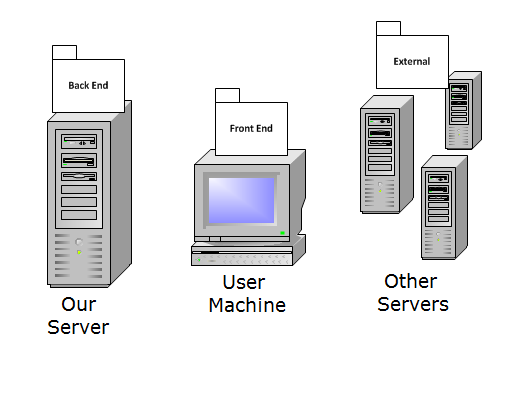
\includegraphics{./img/hardware.png}
\caption{The hardware mapping for our system.}
\end{figure}